\documentclass[a4paper,12pt]{article}

\usepackage[
    left=2cm,
    right=2cm,
    top=3cm,
    bottom=3cm
]{geometry}

\usepackage[utf8]{inputenc}
\usepackage[czech]{babel}
\usepackage[T1]{fontenc}
\usepackage{graphicx}
\usepackage{array}
\usepackage{booktabs}
\usepackage{tabularx}
\usepackage{makecell}
\usepackage{float}
\usepackage{newunicodechar}
\usepackage{url}
\usepackage{siunitx}
\usepackage{listings}
\usepackage{xcolor}
\usepackage{diagbox}
\usepackage{hyperref}
\usepackage{tikz}
\usepackage{pgfplots}
\pgfplotsset{compat=1.18}

\usepackage{fancyhdr}
\pagestyle{fancy}

\fancyhf{}
\fancyhead[L]{SME -- Lab 4: Optické senzory}
\fancyhead[R]{Pavel Pernička}
\fancyfoot[C]{\thepage}

\fancypagestyle{firstpage}{
    \fancyhf{}
    \renewcommand{\headrulewidth}{0pt}
    \renewcommand{\footrulewidth}{0pt}
    \fancyfoot[C]{\thepage}
}

\definecolor{myblue}{RGB}{111,0,248}
\newcommand{\colorcircle}[1]{%
  \tikz[baseline=-0.6ex]\draw[fill=#1,draw=none] (0,0) circle (1.5ex);%
}
\newcommand{\unitC}{\,^\circ\mathrm{C}}
\newcommand{\unitV}{\,\mathrm{V}}
\newcommand{\unitA}{\,\mathrm{A}}
\newcommand{\units}{\,\mathrm{s}}
\newcommand{\unitmin}{\,\mathrm{min}}

\newcommand{\centered}[1]{\begin{tabular}{l} #1 \end{tabular}}

\addto\captionsczech{\renewcommand{\refname}{Seznam použité literatury}}
\addto\captionsczech{\renewcommand{\figurename}{\textbf{Obrázek}}}
\addto\captionsczech{\renewcommand{\tablename}{\textbf{Tabulka}}}
\renewcommand{\lstlistingname}{\textbf{Kód}}

\lstset{
    language=Python,
    basicstyle=\ttfamily\footnotesize,
    keywordstyle=\color{blue},
    commentstyle=\color{gray},
    stringstyle=\color{red},
    numbers=left,
    numberstyle=\tiny\color{gray},
    stepnumber=1,
    breaklines=true,
    frame=single
}

\begin{document}
\thispagestyle{firstpage}

\vspace*{\fill}
\begin{center}
\renewcommand{\arraystretch}{1.75}

\begin{tabularx}{\textwidth}{|X|X|X|}
    \hline
    \multicolumn{1}{|c|}{\rule{0pt}{2.25cm} 
\includegraphics[height=2cm]{img/ctu_logo.png}}
    & \multicolumn{2}{c|}{\makecell{\textbf{KATEDRA MĚŘENÍ}}} \\
    \hline
    \multicolumn{3}{|c|}{\Large \textbf{\centered{Senzory a měření}}} \\
    \hline
    \multicolumn{2}{|X}{\small{Jméno} \newline \textbf{Pavel Pernička}}
    & \multicolumn{1}{|X|}{\small{Datum měření} \newline \textbf{25.2.2026}} \\
    \hline
    {\small{Semestr} \newline \textbf{Letní 2026}}
    & {\small{Ročník} \newline \textbf{2.}}
    & {\small{Datum odevzdání} \newline \textbf{4.3.2026}} \\
    \hline
    \multicolumn{3}{|c|}{\rule{0pt}{1cm}} \\
    \hline
    \multicolumn{1}{|X|}{\small{Číslo úlohy \newline \textbf{4}}}
    & \multicolumn{2}{|p{9cm}|}{\small{Název úlohy \newline \textbf{Optické senzory}}} \\
    \hline
\end{tabularx}

\end{center}
\vspace*{\fill}

\newpage
\pagestyle{fancy}
\section{Úkol 4a. -- Měření parametrů fotodiody}
\subsection{Domácí příprava}
\begin{itemize}
  \item{Jaký je vstupní odpor převodníku I-U dle schématu a jak určíte velikosti proudu $I_{FD1}$ z~napětí $U_{OZ}$? -- Vstupní odpor I-U převodníku je nulový, proud $I_{FD1}=\frac{U_{OZ}}{R_{Z}}$}
  \item{Jak lze určit výstupní odpor zdroje signálu, znáte-li jeho výstupní napětí naprázdno a~proud nakrátko? -- $R_{OUT} = \frac{U_{NAPRÁZDNO}}{I_{NAKRÁTKO}}$}
  \item{Jak lze určit výstupní odpor zdroje signálu na základě změřené zatěžovací charakteristiky? -- zjistíme napětí naprázdno, resp. s velmi malým proudem v charakteristice a vydělíme proudem (téměř) nakrátko, což bude maximální hodnota proudu dosažená v charakteristice}
\end{itemize}

\begin{figure}[H]
\centering
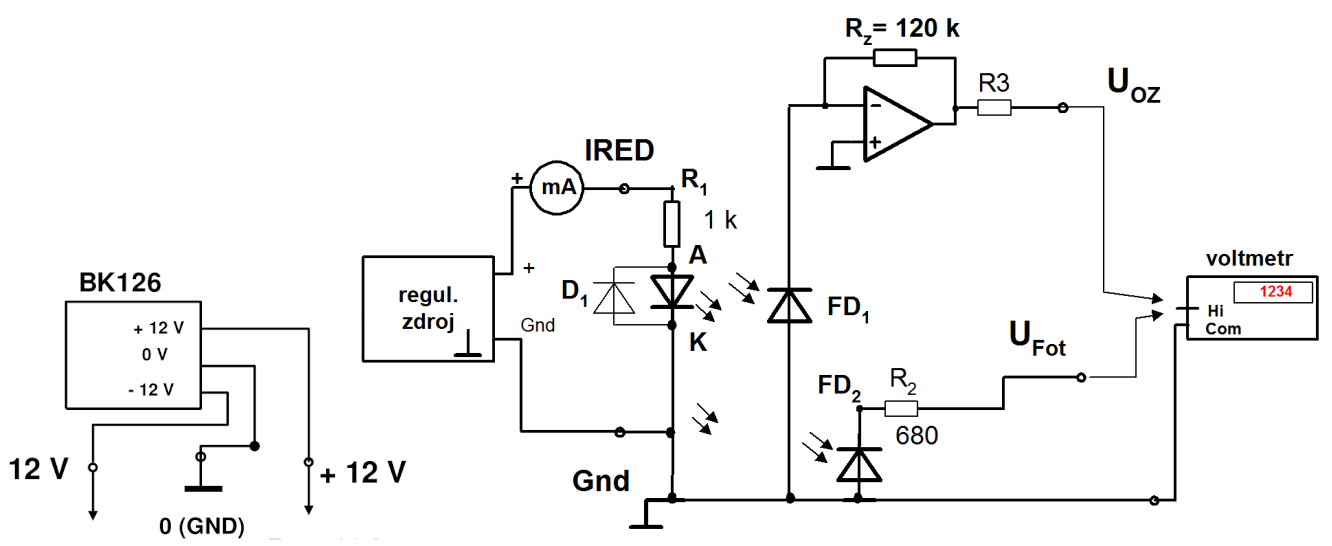
\includegraphics[width=0.90\textwidth]{img/schema.png}
\caption{Schéma zapojení měřeného obvodu}
\label{fig:zapojeni}
\end{figure}

\subsection{Měření výstupního proudu a napětí fotodiody}
\begin{itemize}
  \item Změřte velikost výstupního signálu fotodiody $FD_1$ v členu IL300 v závislosti na velikosti budicího proudu $I_{RED}$ (infračervené diody), jejíž záření dopadá na fotodiodu. Měřte v rozmezí proudu $I_{RED} = 0$ až $12\,\mathrm{mA}$ (např. pro $0$, $4$, $8$, $12\,\mathrm{mA}$). Pro měření proudu nakrátko $I_{FD1}$ využijte převodník proud/napětí s operačním zesilovačem v zapojení dle obr.~1. Naměřené hodnoty $U_{OZ}$ a vypočtené hodnoty proudu $I_{FD1}$ zapište do tabulky.
  \item Pro stejné velikosti budicího proudu $I_{RED}$ jako v předchozím případě určete velikost výstupního napětí naprázdno fotodiody $FD_2$ připojené na výstup $U_{FOT}$ (viz obr.~1). Pro měření použijte číslicový voltmetr se vstupním odporem $\geq 10\,\mathrm{M\Omega}$. Naměřené hodnoty $U_{FOT}$ zapište do tabulky.
\end{itemize}

\begin{table}[H]
\centering
\begin{tabular}{|c|c|c|c|c|}
\hline
$I_{RED}\, [\mathrm{mA}]$ & 0 & 4 & 8 & 12 \\
\hline
$U_{OZ}\, [\mathrm{V}]$ & 0 & 2,75 & 6,08 & 9,45 \\
\hline
$I_{FD1}\, [\mathrm{mA}]$ & 0 & 0,023 & 0,051 & 0,079 \\
\hline
\end{tabular}
\caption{Výstupní signál $U_{FD1}$ v členu IL300 v závislosti na $I_{RED}$}
\end{table}

\begin{table}[H]
\centering
\begin{tabular}{|c|c|c|c|c|}
\hline
$I_{RED}\, [\mathrm{mA}]$ & 0 & 4 & 8 & 12 \\
\hline
$U_{FOT}\, [\mathrm{V}]$ & 0 & -0,44 & -0,47 & -0,49 \\
\hline
\end{tabular}
\caption{Výstupní signál $U_{FOT}$ v závislosti na $I_{RED}$}
\end{table}

\subsection{Určení vnitřního odporu zapojení s fotodiodou}
\begin{itemize}
  \item Určete velikost ochranného rezistoru R3, který se v zapojení chová jako vnitřní odpor zdroje signálu $U_{OZ}.$
\end{itemize}
Zde zvolíme metodu, kdy na svorku $U_{OZ}$ připojíme nastavitelnou odporovou zátěž, kterou postupně zvyšujeme, dokud nám měřené napětí neklesne na polovinu oproti původní hodnotě bez zátěže. Zjištěný odpor je $\mathbf{R_3 = 10\ 690\ \Omega}$.

\section{Úkol 4b. -- Optoelektronické snímače polohy}
\subsection{Domácí příprava}
\begin{itemize}
\item Jaké hlavní nectnosti má jednoduchý optický reflexní snímač polohy? Proč se používá modulace světelného zdroje a průměrování? -- Nevýhodou je závislost na odrazivosti materiálu, náchylnost na okolní osvícení a poměrmě široký vyzařovací úhel. Modulaci používáme, abychom mohli vysílat po krátkou dobu špičkovým výkonem a abychom z přijatého signálu mohli zjistit, že je to ten náš.
\item Co je hlavní výhoda triangulačního snímače vzdálenosti? -- Nezávisí na odrazivosti povrchu.
\item Jak je v triangulačním snímači vzdálenosti zajištěno, že nereaguje na rušivé okolní světlo? -- Pomocí vyhodnocení modulace signálu, případně skrzečočku s band-pass filtrem na specifickou vlnovou délku.
\end{itemize}

\newpage
\subsection{Reflexní snímač s optickými vlákny}
Určete závislost výstupního signálu na vzdálenosti u reflexního snímače s optickými vlákny pro vzdálenost $5\,\mathrm{mm}$ až $300\,\mathrm{mm}$. Velikost kroku volte adaptivně podle změny úrovně výstupního signálu, měření proveďte alespoň v \textbf{šesti bodech}. Hodnoty odečítejte z panelu zesilovače E3X-DA51-N.

\begin{table}[H]
\centering
\begin{tabular}{|c|c|c|c|c|c|c|c|c|}
\hline
Vzdálenost [mm] & 5 & 7 & 10 & 15 & 20 & 30 & 80 & 300 \\
\hline
Hodnota & 3553 & 2620 & 1757 & 1062 & 705 & 364 & 65 & 5 \\
\hline
\end{tabular}
\caption{Naměřená závislost pro reflexní snímač}
\end{table}

\begin{figure}[H]
\centering
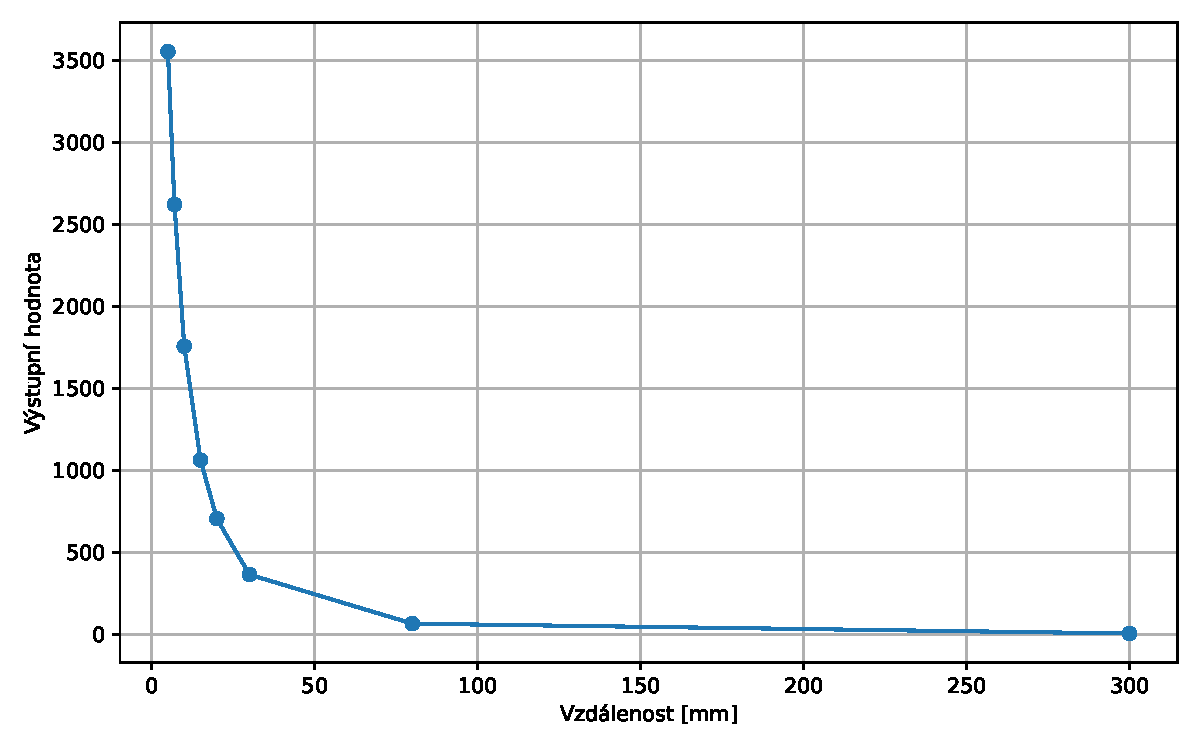
\includegraphics[width=0.8\textwidth]{img/zavislost1.pdf}
\caption{Závislost výstupního signálu na vzdálenosti pro reflexní snímač}
\end{figure}

\newpage
\subsection{Optická závora}
Určete závislost výstupního signálu optické závory se senzorovou hlavou E32~TC16 na stupni jejího zaclonění. Určete převodní konstantu 
\[
k_p = \frac{\Delta x_{cl}}{\Delta N}
\]
závislosti $N = f(\Delta x_{cl})$ ve Vámi zvolené lineární oblasti, měřením ve dvou bodech, kde $x_{cl}$ je velikost posunu clonky v mm a $N$ je údaj na zobrazovači zesilovače E3X-DA51-S.

\begin{table}[h]
\centering
\begin{tabular}{|c|c|c|c|c|c|c|c|}
\hline
Průměr clonky [mm] & 0 & 3.2 & 4.2 & 5.6 & 7.4 & 8.7 & 10,5 \\
\hline
Hodnota $N$ & 3222 & 1536 & 1273 & 560 & 125 & 50 & 0 \\
\hline
\end{tabular}
\caption{Naměřená závislost hodnoty snímače na průměru clonky}
\end{table}

\begin{figure}[H]
\centering
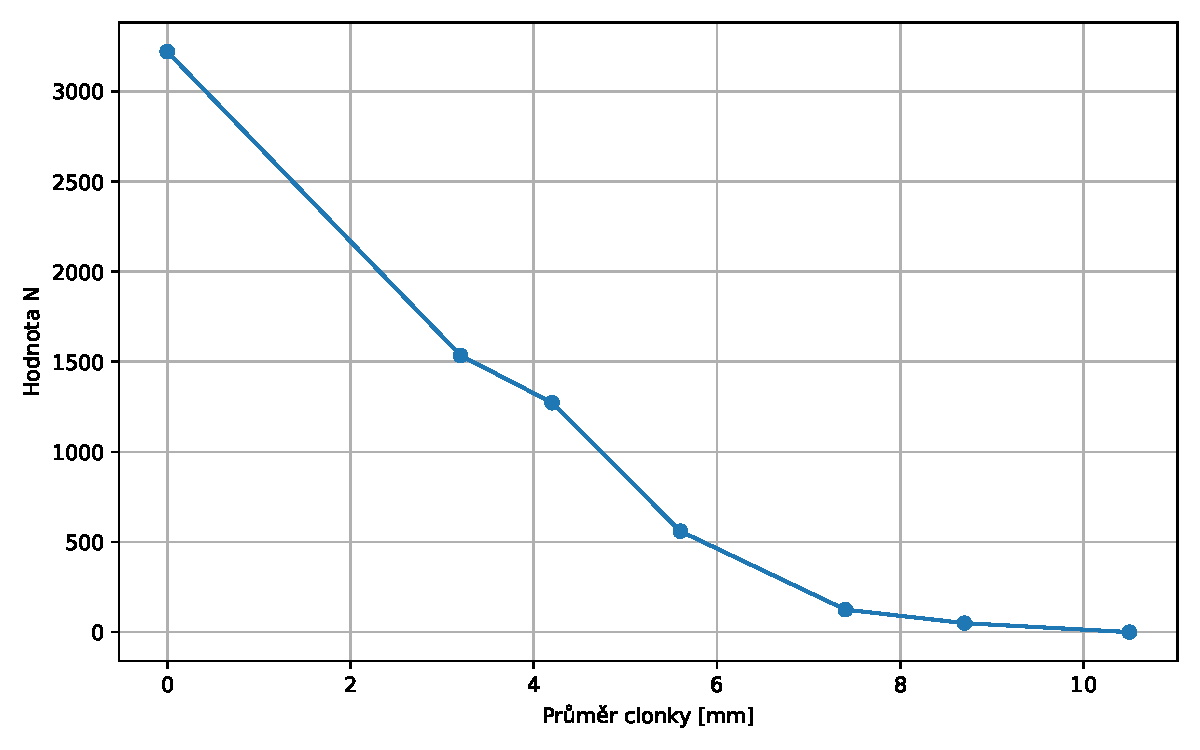
\includegraphics[width=0.8\textwidth]{img/zavislost2.pdf}
\caption{Závislost hodnoty snímače na průměru clonky}
\end{figure}

Pro určení převodní konstanty nejprve normalizujeme průměry clonek na stupeň zakrytí: $Z = \frac{R_N}{10,5}\cdot 100$. Následně dosadíme do vzorečku:
\[
k_p = \frac{\Delta x_{cl}}{\Delta N} = \frac{70.48 - 40}{1273-125} = \frac{30.48}{1148} \approx 0.0266
\]

\newpage
\subsection{Modulace signálu snímače polohy}
Pomocí přípravku s fotodiodou a osciloskopu změřte s jakou frekvencí a střídou je modulován optický signál ve snímačích polohy. Průběh si zaznamenejte.

Určili jsme frekvenci $\mathbf{f = 959\ Hz}$ a duty cycle $\mathbf{12,5\ \%}$

\begin{figure}[H]
\centering
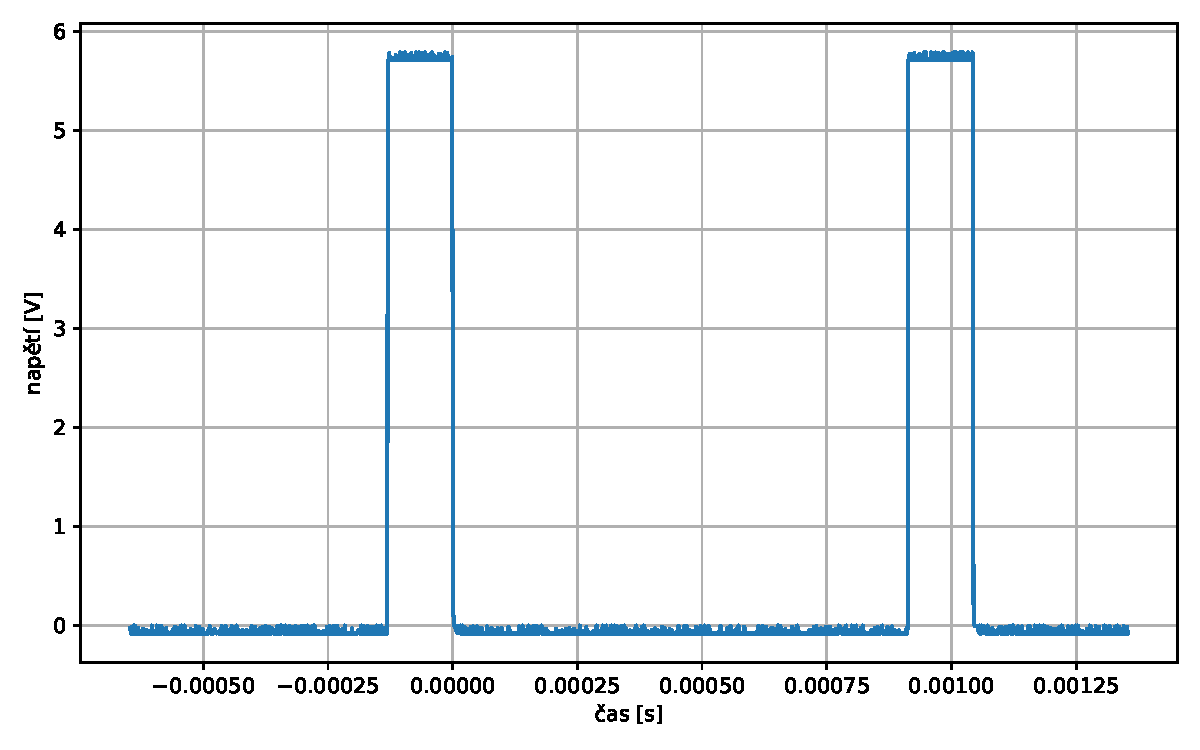
\includegraphics[width=0.8\textwidth]{img/zavislost3.pdf}
\caption{Naměřený průběh signálu z fotodiody namíření na snímač polohy}
\end{figure}

\subsection{Reflexní senzor s polarizovaným světlem}
Seznamte se s funkcí reflexního senzoru s polarizovaným světlem, graficky naznačte princip funkce. Pomocí polarizačního filtru se přesvědčte, že výstupní světlo ze senzoru je polarizované (intenzita světla se mění dle úhlového natočení filtru).

Senzor vysílá světlo v jedné polarizaci. To se na retroreflektoru odrazí v polarizaci otočené o $90°$ a dorazí ke snímači, který má před sebou polarizační filtr, který propouští právěv této polarizaci.

\begin{figure}[H]
\centering
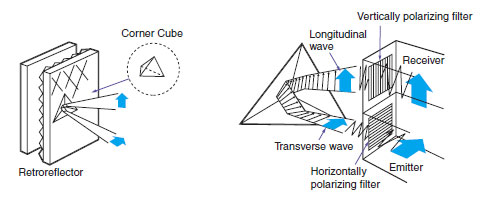
\includegraphics[width=0.7\textwidth]{img/polarizace.png}
\caption{Schéma principu fungování reflexního senzoru s polarizací (zdroj: omron.com)}
\end{figure}

\subsection{Triangulační snímač}
Zjistěte závislost výstupního napětí triangulačního optického snímače Sharp GP2Y0A21YK0F na vzdálenosti bílé odrazné plochy s matným povrchem. Měřte ve vzdálenostech od 5 cm do 30 cm (měřicí vzdálenosti zvolte tak, aby bylo možno Vámi zjištěnou charakteristiku porovnat s~katalogovým údajem.

\begin{table}[H]
\centering
\begin{tabular}{|c|c|c|c|c|c|c|c|}
\hline
Vzdálenost [mm] & 300 & 250 & 200 & 150 & 100 & 50 & 5 \\
\hline
$U_{\text{SENZ}}$ [V] & 0.88 & 1.03 & 1.27 & 1.59 & 2.22 & 3.15 &  \\
\hline
\end{tabular}
\caption{Naměřená závislost výstupního napětí triangulačního senzoru na vzdálenosti}
\end{table}


\begin{figure}[H]
\centering
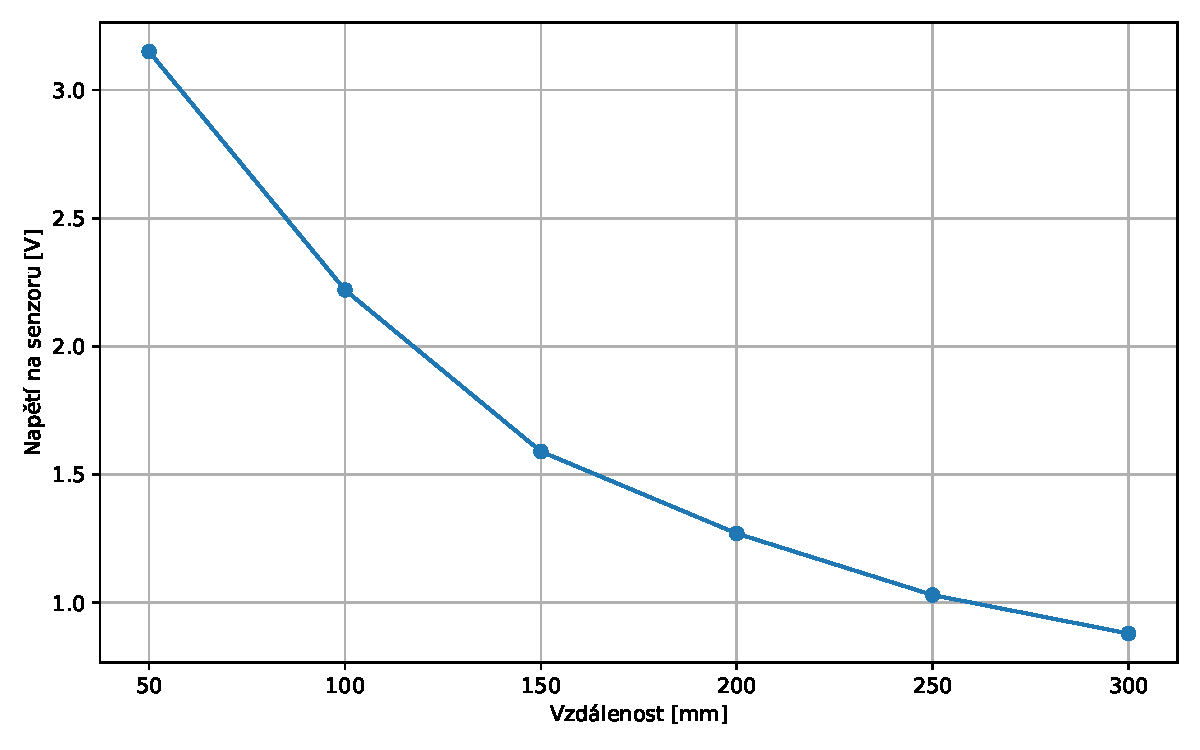
\includegraphics[width=0.8\textwidth]{img/zavislost4.pdf}
\caption{Závislost výstupního napětí triangulačního senzoru na vzdálenosti}
\end{figure}

Srovnání s datasheetem -- Průběh je tvarově téměř totožný, ale naše naměřená napětí jsou cca 3,75x vyšší.
\end{document}
